\newpage
\section{Control systems}
\vspace{-3mm}
\subsection{Introduction}
\vspace{-3mm}

% 4 pages given, 8 sections in total.
% Each section should be roughly 1/2 page long.

% - (I) What is a bioreactor control system?

Homeostasis, defined as the internal regulatory functions of the body to maintain certain conditions constant~\citep{E-Guyton2006, E-Aging2022}, is extremely crucial to living organisms. For example, for humans, the blood pH outside the range between 7.35 and 7.45 can cause death \cite{E-Donaldson2013}. In addition to its significance in maintaining an existing life, homeostasis has great importance in creating a new life: Mammalian cell culture.

In a bioreactor, homeostasis can be achieved by solving the classical problem of tracking the reference signal $r(t)$ in control theory, as shown in Figure \ref{figure:E-1-1-control-system}. A thoroughly designed bioreactor and its constituent control systems will lead to better achievement of the design objectives, which are: (i) How can one achieve the production rate of 100 kg/month? (ii) How can one produce a better quality of meat?

The design of the control system mainly answers the latter question. The former question is rather answered through the overall process diagram, number and sizes of bioreactors, mass inflows and outflows, so will not be tackled in this chapter. Bioreactor control, however, addresses the formation and maintenance of the optimal environment to produce the best quality of meat. Thus, in this chapter, the design of temperature (T), dissolved oxygen (DO) and acidity (pH) control systems are discussed.

\begin{figure}[h]
    \centering
    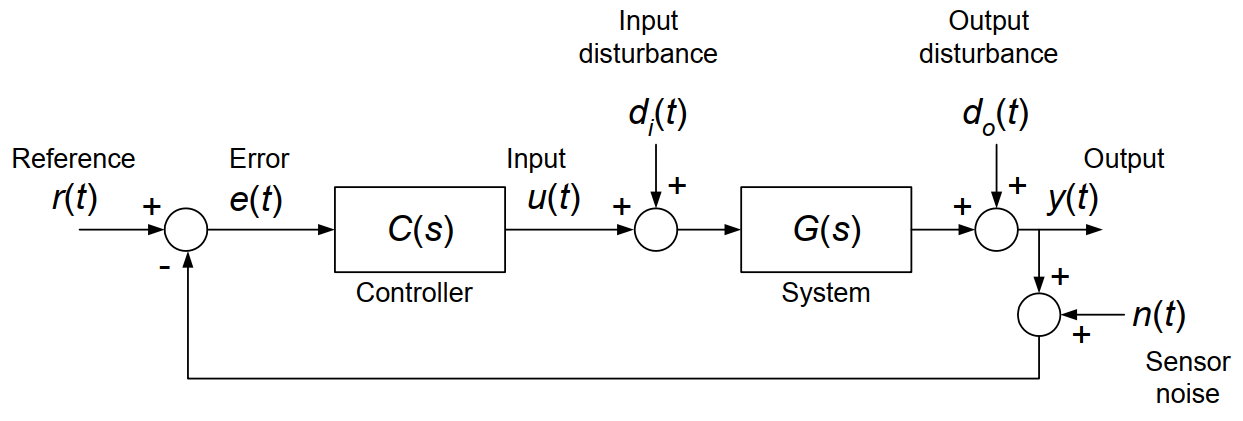
\includegraphics[width=0.75\textwidth]{eunsoo/E-1-1-control-system.png}
    \hfill
    \caption{A schematic of a negative feedback control system \citet{E-Cannon2022}}
    \label{figure:E-1-1-control-system}
\end{figure}

\vspace{-10mm}
\subsection{Temperature control}
\vspace{-3mm}
\subsubsection{Introduction}

% - (I) why consider control systems for temperature?

The body temperature of beef cattle should be maintained at $39.6 \pm 0.1 ^{\circ} C$ \cite{E-Gaughan2014}. To do so, different physical setups of the heat exchanger around the bioreactor will be compared to find the optimal one. Differential equations will be constructed to derive the plant transfer function. Design criteria will be posed with appropriate justification. Different control strategies will be compared to find the optimal one. The design criteria introduced will be used to find control parameters. MATLAB simulations will be used to confirm the validity of the step and impulse responses.

\subsubsection{Methods}

% - (M1) the physical structure of the temperature control system and justification

Various types of heat exchangers used to control the heat in and out of the bioreactor are shown in Figure \ref{figure:E-1-2-heat-exchangers}. The best design choice is (a), the jacketed bioreactor. The logic is as follows: (c) and (d) have the heat exchange inside the bioreactor, causing an intervention in the rotational pathway of the impeller used to stir the meat, and thus adding unnecessary complexity to the design to avoid this; (e) involves taking the meat out of the bioreactor, which firstly may harm the meat cells by pumping and pressurising them above the maximum stress that they they can resist, and secondly has a potential issue of fouling in the pump. One is now left with (a) and (b), but for better heat transfer it is more efficient for the working fluid to cover the entire bioreactor, and for more evenly distributed heat transfer it is better if the inlet and the outlet temperatures of the heat exchanger do not vastly differ. Hence, (a) is the best option.

\begin{figure}[h]
    \centering
    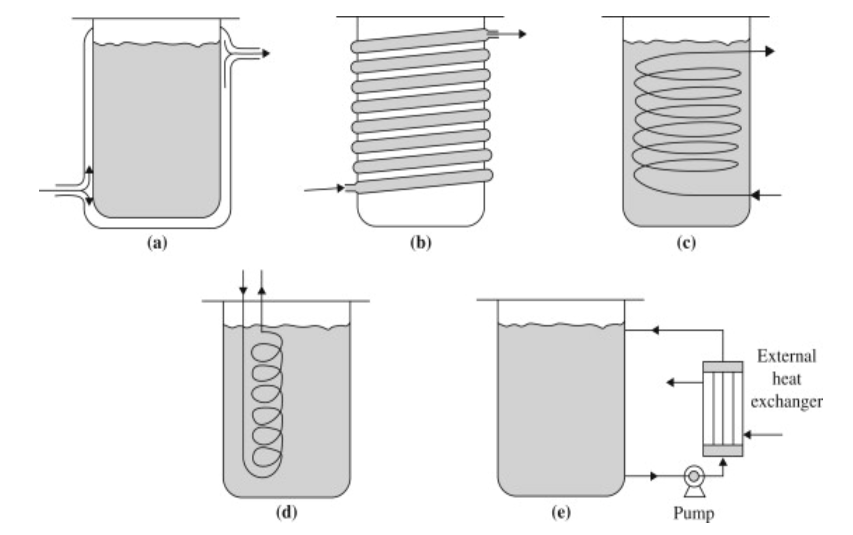
\includegraphics[width=0.5\textwidth]{eunsoo/E-1-2-heat-exchangers.png}
    \hfill
    \caption{Heat exchanger configurations for a bioreactor \cite{E-Doran2013}}
    \label{figure:E-1-2-heat-exchangers}
\end{figure}

\vspace{-5mm}
Theoretically, the heat exchanger's working fluid temperature $T_{fluid}$ controls the bioreactor's internal temperature $T$. Practically, the observer is implemented using a temperature sensor, and the controller is implemented digitally using a computer system, as shown in Figure \ref{figure:E-1-3-digital-control-system}.

\begin{figure}[h]
    \centering
    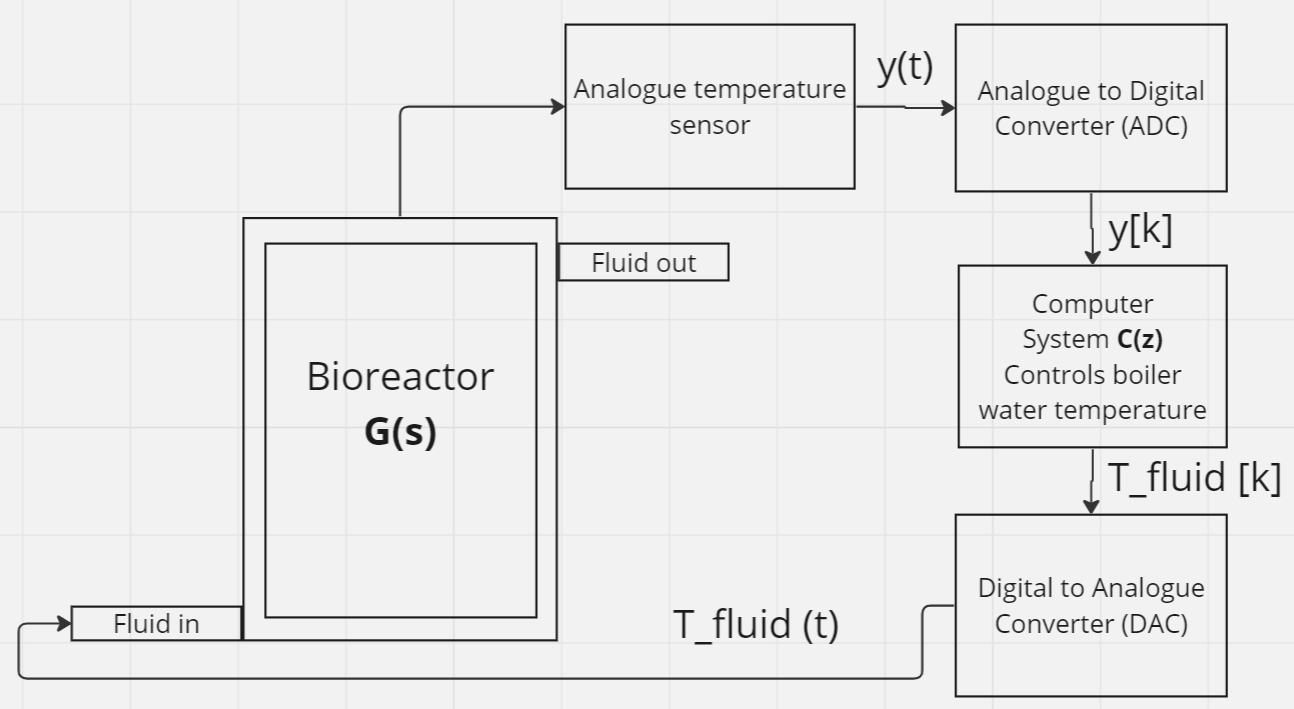
\includegraphics[width=0.6\textwidth]{eunsoo/E-1-3-digital-control-system.png}
    \hfill
    \caption{Practical implementation of the control system}
    \label{figure:E-1-3-digital-control-system}
\end{figure}

\newpage

% - (M2) the mathematical model and transfer function derivation for temperature control

The dynamics over time of temperature ($T$) can be described via the energy balance equation, where $\rho$ is the wet cell density, $V$ is the volume of the bioreactor, $c_p$ is the specific heat capacity, $Q_{met}$ is the metabolic heat generation rate, $h$ is the heat transfer coefficient and $A$ is the area of the bioreactor.

\vspace{-5mm}
\begin{equation}
    \rho V c_p \frac{\partial T}{\partial t} = Q_{met} V - hA(T-T_{fluid})
\end{equation}

The change of variables to perturbations $\Delta T = T(t) - T_{ss}$ and $\Delta T_{fluid} = T_{fluid}(t) - T_{fluid, ss}$ leads to Equation \ref{equation:E-temp-2}. During the entire culturing period ($t>0$) the steady-state assumption ($\frac{\partial \Delta T}{\partial t} = 0$, $\Delta T \approx \Delta T_{fluid} \approx 0$) can be made because otherwise the cells will die due to the violence of homeostasis. This leads to Equation \ref{equation:E-temp-3}. Substituting Equation \ref{equation:E-temp-3} into Equation \ref{equation:E-temp-2} and taking the Laplace transform leads to the desired transfer function, as shown in Equation \ref{equation:E-temp-4}.

\vspace{-5mm}
\begin{equation}
    \rho V c_p \frac{\partial \Delta T}{\partial t} = Q_{met} V - hA(T_{ss} - T_{fluid, ss}) - hA(\Delta T - \Delta T_{fluid})
    \label{equation:E-temp-2}
\end{equation}

\vspace{-10mm}
\begin{equation}
    Q_{met} V - hA(T_{ss} - T_{fluid, ss}) = 0
    \label{equation:E-temp-3}
\end{equation}

\vspace{-10mm}
\begin{equation}
    G(s) = \frac{\Delta T(s)}{\Delta T_{fluid}(s)} = \frac{hA}{\rho V c_p s + hA}
    \label{equation:E-temp-4}
\end{equation}

\subsubsection{Results}

%- (R1) the numerical values of parameters summarised in a table and justification

%- (R2) proposal of design criteria and PID controller implementation

%- (R3) demonstration of the step and impulse responses of the system and the PID controller performance

The wet cell mass of $3.5 \times 10^{-12} \ kg/cell$ and the cell diameter of $295 \times 10^{-6} \ m$ \cite{E-Furuhashi2021} are used to calculate the density so that $\rho = 0.26 \ kg/m^3$. The bioreactor height of $2 \ m$ and the bioreactor diameter of $2.1 \ m$, are used to calculate the area and the volume of the bioreactor so that $A = 20.12 \ m^2$ and $V = 6.93 \ m^3$. The yield of the final product to the wet cell $\eta = 0.5$ is used along with $c_{p, cell} = 3.440 \ kJ kg^{-1} K^{-1}$ \cite{E-Fellows2009} and $c_{p, water} = 4.180 \ kJ kg^{-1} K^{-1}$ to linearly interpolate the specific enthalpy as shown in Equation \ref{equation:E-temp-5}. The heat transfer coefficient is assumed to be $h = 0.5 \ kW m^{-2} K^{-1}$. Substituting these values in, the plant transfer function is derived as shown in Equation \ref{equation:E-temp-6}.

\vspace{-5mm}
\begin{equation}
    c_p = \eta c_{p, cell} + (1-\eta) c_{p, water} = 3.810 \ kJ kg^{-1} K^{-1}
    \label{equation:E-temp-5}
\end{equation}

\vspace{-10mm}
\begin{equation}
    G(s) = \frac{10.06}{6.872 s + 10.06}
    \label{equation:E-temp-6}
\end{equation}

The design of the controller is often done by setting the gain margin (GM) or the phase margin (PM) of $C(s)G(s)$ at a chosen frequency. The best design criterion is $PM = 60 ^{\circ}$ at $\omega = 4.16 \ rad/s$. The logic is as follows: the rise time of the plant's step response, defined as the time taken from 10\% to 90\% of the steady-state value, is $\Delta t = 1.58 - 0.07 = 1.51 \ s$, as it is also visible from Figure \ref{figure:E-1-4-step-and-impulse}. The rise time can be viewed as the mean time taken for the bioreactor to respond to the heat exchanger, and hence the period. The operating frequency is then $\omega = 2\pi / \Delta t = 4.16 \ rad/s$.

Practically, there is a higher chance of acceleration or delay in heating and cooling than a sudden overheating or underheating. Thus, one may be more concerned with the phase margin that relates to unexpected phase lags $\angle G(j \omega)$ than the gain margin that relates to unexpected magnitude deviations $|G(j \omega)|$. An acceptable rule of thumb is $PM = 60 ^{\circ}$, so one reaches the posed criterion.

One of the most commonly used controllers in the process control industry is proportional-differentiator-integral (PID). The engineer can use the above criterion along with the condition that "the low-frequency asymptote of the Nyquist on the $M=1$ line" \cite{E-Cannon2022-2}, which means the unity D.C. gain $\frac{Y(s)}{R(s)} = 1$ and thus zero steady-state error. Through this, one can find the three controller gains in $C(s) = K_p + \frac{K_i}{s} + K_d s$.

\begin{figure}[h]
    \centering
    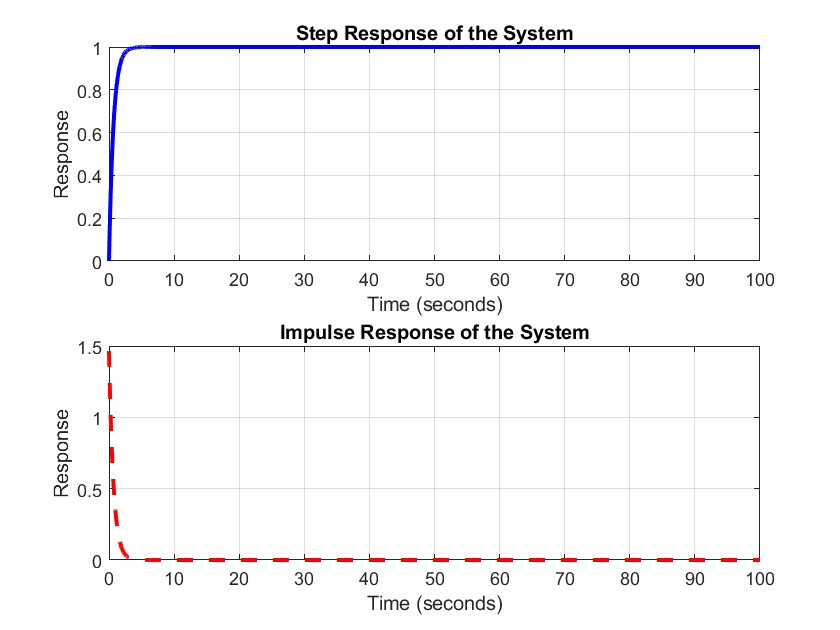
\includegraphics[width=0.7\textwidth]{eunsoo/E-1-4-step-and-impulse.jpg}
    \hfill
    \caption{The step and impulse responses of the plant}
    \label{figure:E-1-4-step-and-impulse}
\end{figure}

\vspace{-10mm}
\subsubsection{Discussion}
- (D) discussion of how my choices led to better achievement of the final objectives, compared to other control strategies

% TESTING WHERE TO PUT BIBLIOGRAPHY
% \begingroup\onehalfspacing
% {\small
% %\renewcommand{\section}[2]{}
% \begin{multicols}{2}
% \bibliographystyle{unsrt}
% %\bibliographystyle{elsarticle-num}
% % \bibliographystyle{elsarticle-harv}
% % \bibliographystyle{elsarticle-num-names}
% % \bibliographystyle{model1a-num-names}
% % \bibliographystyle{model1b-num-names}
% % \bibliographystyle{model1c-num-names}
% % \bibliographystyle{model1-num-names}
% % \bibliographystyle{model2-names}
% % \bibliographystyle{model3a-num-names}
% % \bibliographystyle{model3-num-names}
% % \bibliographystyle{model4-names}
% % \bibliographystyle{model5-names}
% % \bibliographystyle{model6-num-names}
% \bibliography{mybib.bib}
% \end{multicols}}
% \endgroup